\section{Introduction}

Sequential decision-making is a field that examines how agents make a series of interconnected decisions to achieve specific goals. 
In such scenarios, the optimal choice of actions often depends on the context, and the correct path forward is rarely obvious. 
Decisions are complicated further by their long-term consequences: actions that may appear suboptimal in the short term can be strategically vital for accomplishing broader objectives.
\begin{figure}[H]
    \centering
    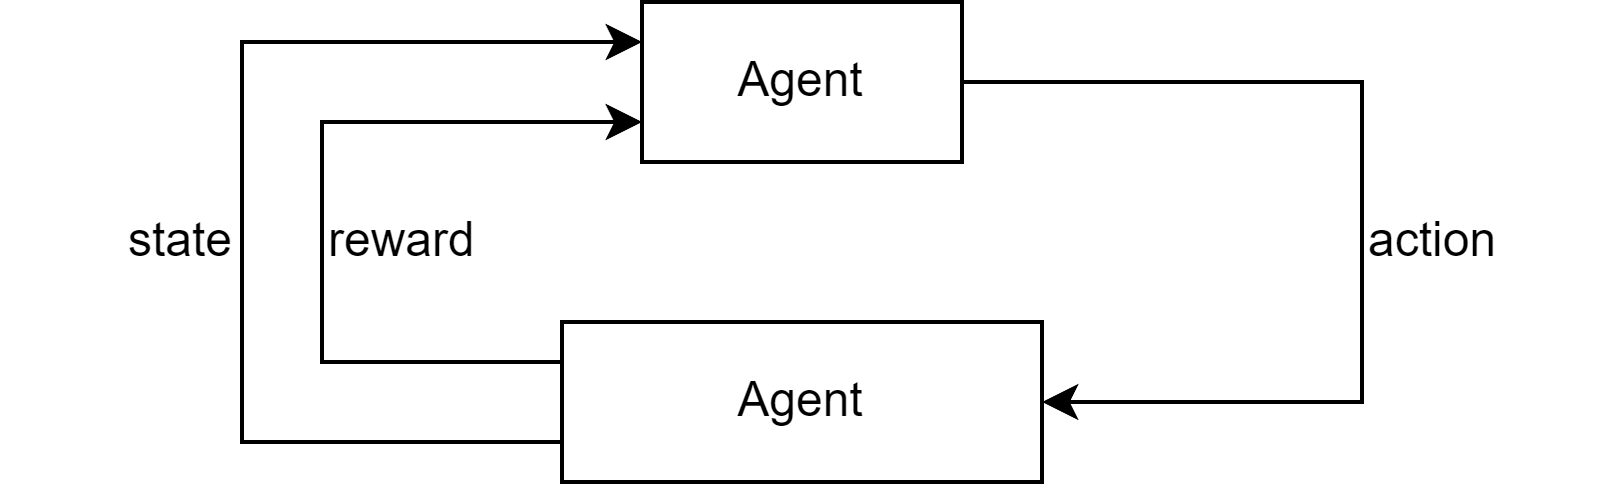
\includegraphics[width=0.75\linewidth]{images/rl.png}
    \caption{Agent-environment interface}
\end{figure}
\noindent This interaction unfolds at discrete time steps $t = 0, 1, 2, \dots$, and follows a structured cycle:
\begin{enumerate}
    \item \textit{State observation and action selection}: the agent observes the current state $S_t \in \mathcal{S}$ and selects an action $A_t \in \mathcal{A}(S_t)$ based on that state.
    \item \textit{Feedback and transition}: the environment responds by providing a reward $R_{t+1} \in \mathcal{R}$ and transitioning to a new state $S_{t+1} \in \mathcal{S}$ as a result of the agent's action.
\end{enumerate}
\begin{figure}[H]
    \centering
    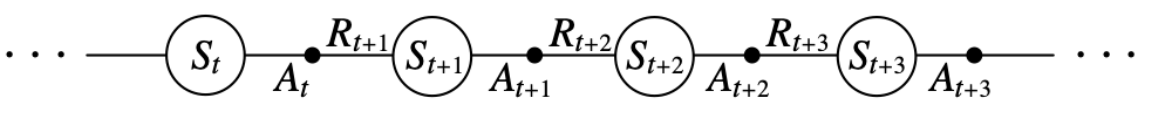
\includegraphics[width=0.75\linewidth]{images/rl1.png}
    \caption{Agent-environment interaction}
\end{figure}